
%%%%%%%%%%%%%%%%%%%%%%%%%%%%% Define Article %%%%%%%%%%%%%%%%%%%%%%%%%%%%%%%%%%
\documentclass[conference]{IEEEtran}
%%%%%%%%%%%%%%%%%%%%%%%%%%%%%%%%%%%%%%%%%%%%%%%%%%%%%%%%%%%%%%%%%%%%%%%%%%%%%%%

%%%%%%%%%%%%%%%%%%%%%%%%%%%%% Using Packages %%%%%%%%%%%%%%%%%%%%%%%%%%%%%%%%%%
\usepackage{geometry}
\usepackage{amssymb}
\usepackage{amsmath}
\usepackage{amsthm}
\usepackage{empheq}
\usepackage{mdframed}
\usepackage{booktabs}
\usepackage{lipsum}
\usepackage{color}
\usepackage{psfrag}
\usepackage{pgfplots}
\usepackage{bm}
\usepackage[spanish]{babel}
\usepackage[utf8]{inputenc} % Codificación UTF-8
\usepackage{amsmath}        % Soporte para ecuaciones matemáticas
\usepackage{graphicx}       % Manejo de imágenes
\usepackage{hyperref}       % Hipervínculos
\usepackage{caption}        % Formato para figuras
\usepackage{multirow}
\usepackage{subcaption}
\usepackage{biblatex}
\usepackage{csquotes}
\usepackage{bookmark}
\usepackage{array}
\usepackage[T1]{fontenc}
\usepackage{lmodern}
\usepackage{amsfonts}
\usepackage{epstopdf}
\usepackage[table]{xcolor}

%%%%%%%%%%%%%%%%%%%%%%%%%%%%%%%%%%%%%%%%%%%%%%%%%%%%%%%%%%%%%%%%%%%%%%%%%%%%%%%

% Other Settings

%%%%%%%%%%%%%%%%%%%%%%%%%% Page Setting %%%%%%%%%%%%%%%%%%%%%%%%%%%%%%%%%%%%%%%
\geometry{a4paper, margin=1in}

%%%%%%%%%%%%%%%%%%%%%%%%%% Define some useful colors %%%%%%%%%%%%%%%%%%%%%%%%%%
\definecolor{ocre}{RGB}{243,102,25}
\definecolor{mygray}{RGB}{243,243,244}
\definecolor{deepGreen}{RGB}{26,111,0}
\definecolor{shallowGreen}{RGB}{235,255,255}
\definecolor{deepBlue}{RGB}{61,124,222}
\definecolor{shallowBlue}{RGB}{235,249,255}
%%%%%%%%%%%%%%%%%%%%%%%%%%%%%%%%%%%%%%%%%%%%%%%%%%%%%%%%%%%%%%%%%%%%%%%%%%%%%%%

%%%%%%%%%%%%%%%%%%%%%%%%%% Define an orangebox command %%%%%%%%%%%%%%%%%%%%%%%%
\newcommand\orangebox[1]{\fcolorbox{ocre}{mygray}{\hspace{1em}#1\hspace{1em}}}
%%%%%%%%%%%%%%%%%%%%%%%%%%%%%%%%%%%%%%%%%%%%%%%%%%%%%%%%%%%%%%%%%%%%%%%%%%%%%%%

%%%%%%%%%%%%%%%%%%%%%%%%%%%% English Environments %%%%%%%%%%%%%%%%%%%%%%%%%%%%%
\newtheoremstyle{mytheoremstyle}{3pt}{3pt}{\normalfont}{0cm}{\rmfamily\bfseries}{}{1em}{{\color{black}\thmname{#1}~\thmnumber{#2}}\thmnote{\,--\,#3}}
\newtheoremstyle{myproblemstyle}{3pt}{3pt}{\normalfont}{0cm}{\rmfamily\bfseries}{}{1em}{{\color{black}\thmname{#1}~\thmnumber{#2}}\thmnote{\,--\,#3}}
\theoremstyle{mytheoremstyle}
\newmdtheoremenv[linewidth=1pt,backgroundcolor=shallowGreen,linecolor=deepGreen,leftmargin=0pt,innerleftmargin=20pt,innerrightmargin=20pt,]{theorem}{Theorem}[section]
\theoremstyle{mytheoremstyle}
\newmdtheoremenv[linewidth=1pt,backgroundcolor=shallowBlue,linecolor=deepBlue,leftmargin=0pt,innerleftmargin=20pt,innerrightmargin=20pt,]{definition}{Definition}[section]
\theoremstyle{myproblemstyle}
\newmdtheoremenv[linecolor=black,leftmargin=0pt,innerleftmargin=10pt,innerrightmargin=10pt,]{problem}{Problem}[section]
%%%%%%%%%%%%%%%%%%%%%%%%%%%%%%%%%%%%%%%%%%%%%%%%%%%%%%%%%%%%%%%%%%%%%%%%%%%%%%%

%%%%%%%%%%%%%%%%%%%%%%%%%%%%%%% Plotting Settings %%%%%%%%%%%%%%%%%%%%%%%%%%%%%
\usepgfplotslibrary{colorbrewer}
\pgfplotsset{width=8cm,compat=1.9}
%%%%%%%%%%%%%%%%%%%%%%%%%%%%%%%%%%%%%%%%%%%%%%%%%%%%%%%%%%%%%%%%%%%%%%%%%%%%%%%

%%%%%%%%%%%%%%%%%%%%%%%%%%%%%%% Title & Author %%%%%%%%%%%%%%%%%%%%%%%%%%%%%%%%
\author{\IEEEauthorblockN{Brayan Joanne Ballesteros Meza, Brayhan Steven Delgado Rueda, Daniel Fernando Aranda Contreras,\\ Jonathan Stiven Murcia Suarez}
\IEEEauthorblockA{Escuela E3T, Universidad Industrial de Santander\\
Correo electrónico: \{brayan2222069, brayan2212088, daniel2221648, jonathan2225092\}@correo.uis.edu.co}}

%%%%%%%%%%%%%%%%%%%%%%%%%%%%%%%%%%%%%%%%%%%%%%%%%%%%%%%%%%%%%%%%%%%%%%%%%%%%%%%
    \begin{document}
        % Título
        \title{\uppercase{modelado de señales periódicas discretas y continuas con la Serie de Fourier}}
        \maketitle
        % Resumen
        % Palabras clave        
        \begin{IEEEkeywords}
            Mediciones Eléctricas,
            Análisis de Sistemas,
            Tensión RMS,
            Compensación de Carga,
            Potencia Activa.
        \end{IEEEkeywords}
        

        \section{Introducción}
        Para realizar esta actividad se debe considerar que la señal de tensión es una onda cuadrada de amplitud 100 [V] con frecuencia fundamental 400 Hz. Esta señal se muestrea con tres diferentes frecuencias de muestreo: \( f_{m1} = 1,600 \) Hz, \( f_{m2} = 3,200 \) Hz y \( f_{m3} = 6,400 \) Hz.
        
        \section{Modelos de la Serie de Fourier de las Señales Discretas}
        \subsection{Señal 1: \texorpdfstring{$f_{m1} = 1,600$ Hz}{f_m1 = 1,600 Hz}}
        \begin{center}
            $v_1[n]= \displaystyle  100\sqrt{2} \cos\left(\frac{\pi}{2}n-\frac{\pi}{4} \right)$
        \end{center}

        \subsection{Señal 2: \texorpdfstring{$f_{m2} = 3,200$ Hz}{f_m2 = 3,200 Hz}}
        \begin{center}
            $v_2[n]=\displaystyle  92.3880 \sqrt{2} \cos\left(\frac{\pi}{8}n-\frac{3\pi}{8}\right)$ \\ 
            \vspace{0.2cm}
            $+38.2683 \sqrt{2} \cos\left(\frac{3\pi}{8}n-\frac{\pi}{8}\right)$
        \end{center}

        \subsection{Señal 3: \texorpdfstring{$f_{m3} = 6,400$ Hz}{f_m3 = 6,400 Hz}}
        \begin{center}
            $v_3[n]=\displaystyle 90.6127\sqrt{2}\cos\left(\frac{\pi}{8}n-\frac{7\pi}{16}\right)$ \\ 
            \vspace{0.2cm}
            $+31.8190\sqrt{2}\cos\left(\frac{3\pi}{8}n-\frac{5\pi}{16}\right)$ \\ 
            \vspace{0.2cm}
            $+21.2608\sqrt{2}\cos\left(\frac{5\pi}{8}n-\frac{3\pi}{16}\right)$ \\ 
            \vspace{0.2cm}
            $+18.0240\sqrt{2}\cos\left(\frac{7\pi}{8}n-\frac{\pi}{16}\right)$
        \end{center}

        \section{Modelos de las Señales Continuas}
        \subsection{Señal 1: $f_{m1} = 1,600$ Hz}
        \begin{center}
            $v_1(t)= \displaystyle  100\sqrt{2} \cos\left(800\pi t-\frac{\pi}{4} \right)$
        \end{center}

        \subsection{Señal 2: $f_{m2} = 3,200$ Hz}
        \begin{center}
            $v_2(t)= \displaystyle  92.3880 \sqrt{2} \cos\left(800\pi t-\frac{3\pi}{8}\right)$ \\ 
            \vspace{0.2cm}
            $+38.2683 \sqrt{2} \cos\left(2400\pi t-\frac{\pi}{8}\right)$
        \end{center}

        \subsection{Señal 3: $f_{m3} = 6,400$ Hz}
        \begin{center}
            $v_3(t)=\displaystyle 90.6127\sqrt{2}\cos\left(800\pi t-\frac{7\pi}{16}\right)$ \\ 
            \vspace{0.2cm}
            $+31.8190\sqrt{2}\cos\left(2400\pi t-\frac{5\pi}{16}\right)$ \\ 
            \vspace{0.2cm}
            $+21.2608\sqrt{2}\cos\left(4000\pi t-\frac{3\pi}{16}\right)$ \\ 
            \vspace{0.2cm}
            $+18.0240\sqrt{2}\cos\left(5600\pi t-\frac{\pi}{16}\right)$
        \end{center}

        \begin{figure}[ht!] % 'h' indica que la imagen se coloca aquí
            \centering
            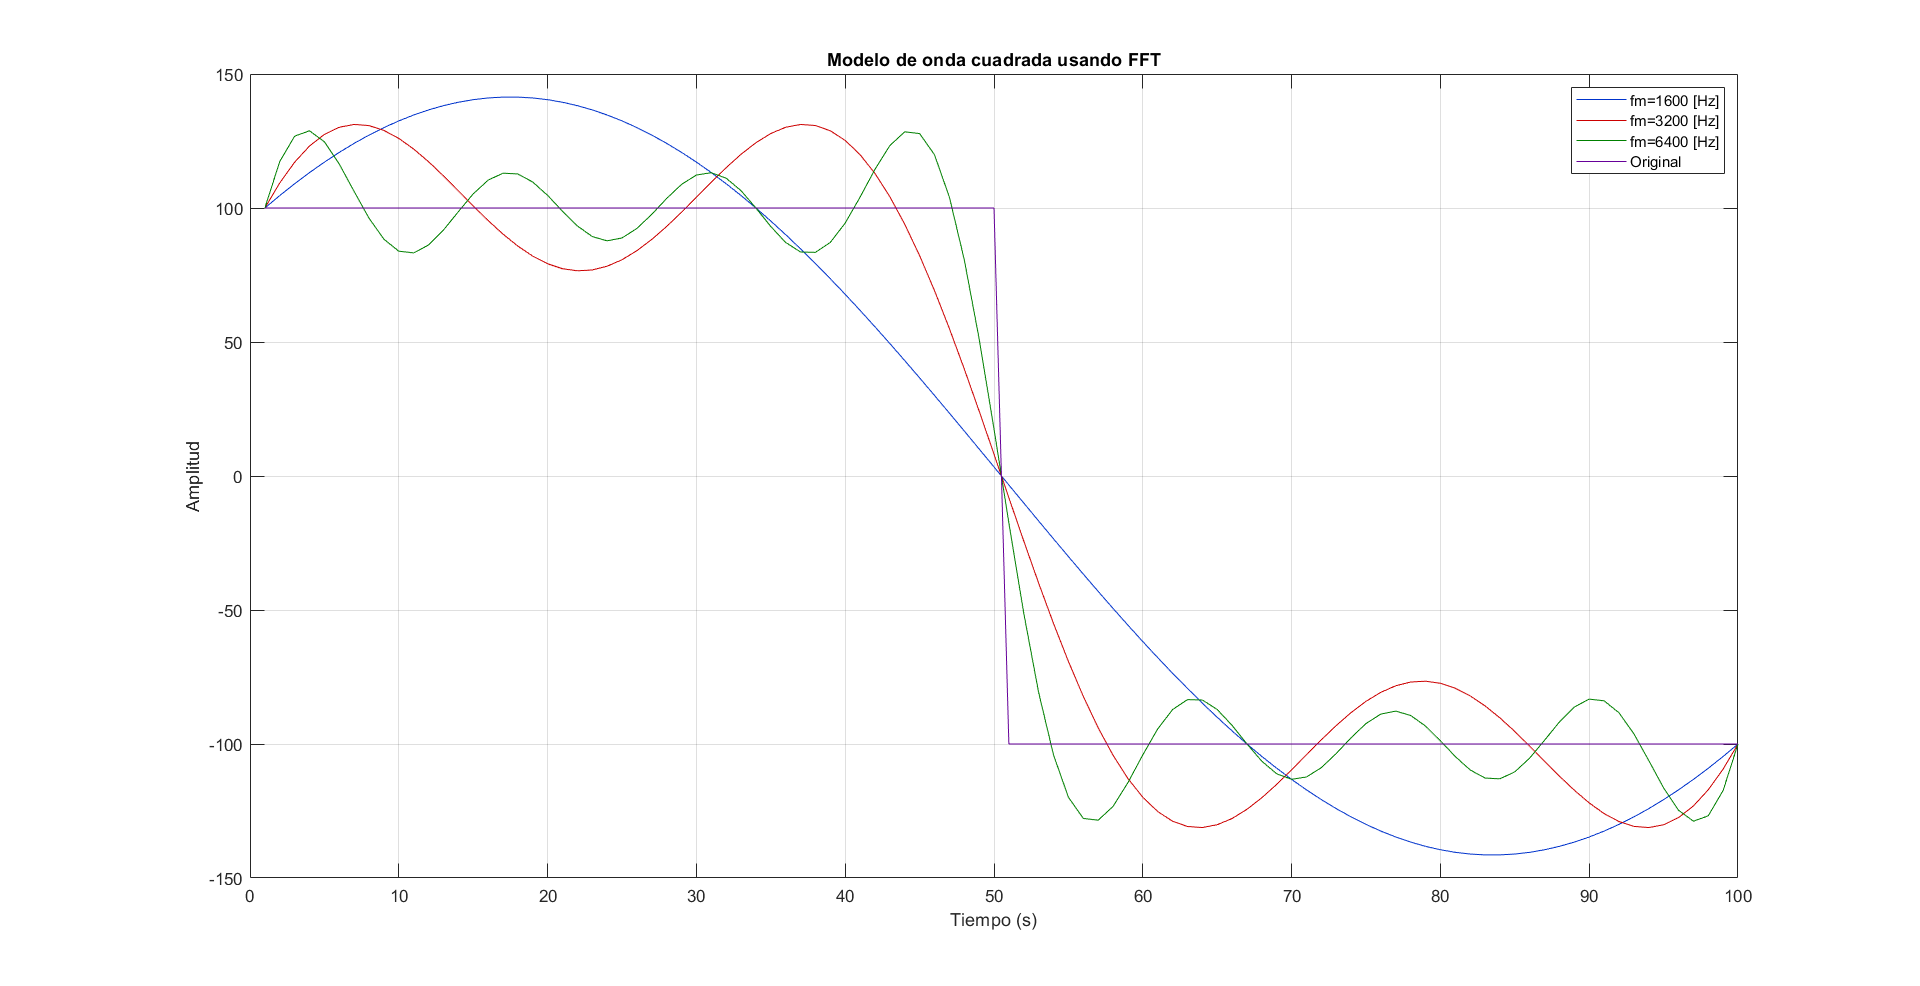
\includegraphics[width=0.48\textwidth]{img/prac8.png} % Cambia la ruta a tu imagen
            \caption{Resultados con el modelo del tiempo.}
            \label{fig:hoja}
        \end{figure}

        \section{Cálculo de Parámetros}
        \subsection{Valor Eficaz, Valor Máximo y Factores de Forma y de Cresta}
        Los valores eficaces \( V_{rms} \), los valores máximos \( V_{max} \), los factores de forma y de cresta para las tres señales continuas se calculan usando las fórmulas estándar de análisis de señales.
        
        \subsection{Errores de Estimación}
        Determinar el error de estimación respecto a la señal cuadrada original implica comparar estos valores con los correspondientes valores para la señal cuadrada original. se tiene en la cuadrada original que $V_{rms}=100[Vrms]$, $FF = 1$ y el $FC=1$.
        A continuacion se presentan los resultados en el modelo del "tiempo" donde t es un vector de 100 valores de 0 hasta $\frac{1}{f_{fundamental}}-\frac{1}{f_{m1}}$ sin embargo en el \textbf{verdadero dominio del tiempo el error es 0\%} para los valores rms, el factor de cresta y el factor de forma puesto que el vector t debe tener valores infinitos en el intervalo del periodo puesto que es el dominio real del tiempo. 
        \begin{table}[h!]
            \centering
            \caption{Valores RMS y errores porcentuales}
            \begin{tabular}{|c|c|c|}
            \hline
            \textbf{Señal} & \textbf{RMS} & \textbf{Error RMS (\%)} \\ \hline
            1 & 109.9966 & 9.9966 \\ \hline
            2 & 104.3163 & 4.3163 \\ \hline
            3 & 102.0001 & 2.0001 \\ \hline
            \end{tabular}
            \label{tabla_rms}
        \end{table}
        \begin{table}[h!]
            \centering
            \caption{Factores de cresta y errores porcentuales}
            \begin{tabular}{|c|c|c|}
            \hline
            \textbf{Señal} & \textbf{FC} & \textbf{Error FC (\%)} \\ \hline
            1 & 1.2853 & 7.3814 \\ \hline
            2 & 1.2576 & 28.5324 \\ \hline
            3 & 1.2629 & 26.2915 \\ \hline
            \end{tabular}
            \label{tabla_factores_fc}
        \end{table}

        \begin{table}[h!]
            \centering
            \caption{Factores de forma y errores porcentuales}
            \begin{tabular}{|c|c|c|}
            \hline
            \textbf{Señal} & \textbf{FF} & \textbf{Error FF (\%)} \\ \hline
            1 & 1.4213 & 7.3814 \\ \hline
            2 & 1.4027 & 9.8425 \\ \hline
            3 & 1.0983 & 9.4241 \\ \hline
            \end{tabular}
            \label{tabla_factores_ff}
        \end{table}
        
        \section{Muestreo de la Señal Continua}
        Para comenzar, se parte de una señal periódica continua, en este caso una onda cuadrada de 100 V con una frecuencia fundamental de 400 Hz. Esta señal se muestrea a distintas frecuencias: 1,600 Hz, 3,200 Hz y 6,400 Hz. El muestreo consiste en tomar valores de la señal a intervalos regulares, generando una secuencia de muestras discretas. Según el teorema de Nyquist, la frecuencia de muestreo debe ser al menos el doble de la frecuencia máxima de la señal para evitar el aliasing, que puede distorsionar la reconstrucción.
        
        \section{Transformada de Fourier Discreta (TFD)}
        Una vez que la señal ha sido muestreada, se aplica la Transformada de Fourier Discreta (TFD) para obtener su representación en el dominio de la frecuencia. La TFD descompone la señal en componentes sinusoidales, permitiendo calcular los coeficientes espectrales como la amplitud y fase que forman la Serie de Fourier discreta. Estos coeficientes contienen la información necesaria para reconstruir la señal.
        
        \section{Reconstrucción de la Señal Continua}
        Con los coeficientes obtenidos a partir de la TFD, se utiliza la fórmula de la Serie de Fourier continua para reconstruir una versión aproximada de la señal original.
        \[
        x[n] = \sum_{k} (X_k \cdot e^{j 2 \pi k f_0 n})
        \]
        Esta reconstrucción se realiza evaluando la suma de armónicos con una resolución temporal mayor, lo que permite obtener una forma de onda continua, suave y más fiel a la original.
        
        \section{Filtrado y Suavizado}
        Para optimizar la calidad de la señal reconstruida y suprimir las componentes de alta frecuencia no deseadas que pueden surgir por un muestreo insuficiente, se emplea un filtro pasa-bajos. Este filtro permite conservar únicamente las frecuencias fundamentales presentes en la señal original, eliminando el ruido espectral y mejorando la suavidad y precisión de la forma de onda resultante.
        
        \section{Evaluación del Modelo}
        A medida que aumenta la frecuencia de muestreo y se consideran más armónicos en la reconstrucción, la señal obtenida se aproxima más a la original. La validez del modelo se puede evaluar comparando parámetros como el valor RMS, el valor pico, el factor de forma (FF) y el factor de cresta (FC), lo cual permite cuantificar el nivel de error y la fidelidad de la reconstrucción.
        
        \end{document}  


        